% Cover letter using letter.cls
\documentclass[a4paper]{scrreprt} 
%\usepackage{helvetica} % uses helvetica postscript font (download helvetica.sty)
%\usepackage{newcent}   % uses new century schoolbook postscript font 
\usepackage[utf8]{inputenc}
\usepackage{graphicx}
\usepackage{amsmath}
\usepackage{eurosym}
\usepackage{cite}
% the following commands control the margins:
%\topmargin=-1in    % Make letterhead start about 1 inch from top of page 
%\textheight=8.5in    % text height can be bigger for a longer letter
%\oddsidemargin=0pt   % leftmargin is 1 inch
%\textwidth=6.5in     % textwidth of 6.5in leaves 1 inch for right margin
\title{Implementing a temperature and humidity sensor network for the nEDM
experiment setup}
\author{Wenwen Chen, Rainer Schönberger}
\begin{document}
\maketitle
\tableofcontents
\input{Concept}
\section{Features}
\section{Sensors}
\subsection{TSIC 506F}
For temperature measurements, we use the TSIC 506F temperature sensor
integrated circuit. At a relatively low price of about \EUR{7} per device, it
is able to deliver very high accuracy (see table \ref{tab:tsic}).\\
The temperature is converted to a digital value, which is sent out over a
proprietary one wire protocol variant, called \emph{ZAC-Wire} (details see section \ref{chap:zac}).\\
In order to minimize soldering heat, which would influence the calibration, we used the TO92 packaged sensor.
\begin{table}[Hh!]
	\centering
	\begin{tabular}{| r | c |}
		\hline
		Temperature range & $-10\,^{\circ}\mathrm{C}$ to $-10\,^{\circ}\mathrm{C}$\\
		\hline
		Calibrated accuracy & $\pm 0.1\,\mathrm{K}$  \\
		\hline
		Resolution & $0.034\,\mathrm{K}$  \\
		\hline
	\end{tabular}
	\caption{TSIC 506F specs}
	\label{tab:tsic}
\end{table}
\subsection{HYT271}
\section{Logical design}
\begin{figure}
	\centering
	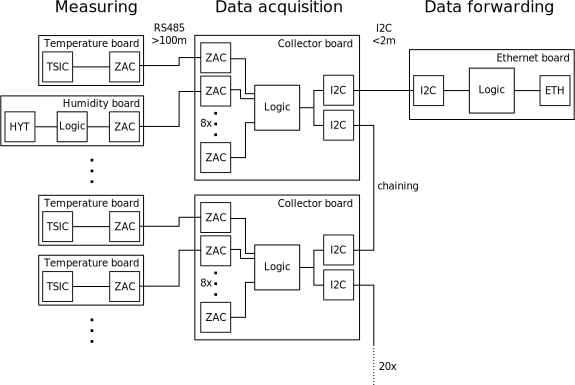
\includegraphics[width=0.9\textwidth]{img/plan2.pdf}
	\caption{Network topology}
	\label{fig:topo}
\end{figure}
\section{Protocols}
\subsection{ZAC}\label{chap:zac}
\begin{figure}
	\centering
	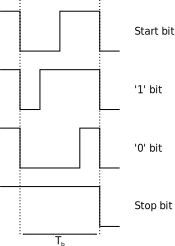
\includegraphics[width=0.3\textwidth]{img/zac_bits.pdf}
	\caption{ZAC protocol signal interpretation}
	\label{fig:zac}
\end{figure}
\begin{figure}
	\centering
	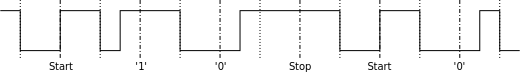
\includegraphics[width=0.9\textwidth]{img/zac_example.pdf}
	\caption{ZAC protocol example}
	\label{fig:zacexample}
\end{figure}
\subsection{I2C}
\subsection{RS485}
\input{Implementation}
\section{Temperature board}
\begin{figure}
	\centering
	\includegraphics[width=0.6\textwidth]{img/schem_temperature_board.pdf}
	\caption{Temperature board schematic}
	\label{fig:schem_temp}
\end{figure}
\section{Humidity board}
\subsection{Hardware}
\begin{figure}
	\centering
	\includegraphics[width=0.8\textwidth]{img/schem_humidity_board.pdf}
	\caption{Humidity board schematic}
	\label{fig:schem_hum}
\end{figure}
\subsection{Software}
\section{Collector board}
The collector board decodes the ZAC protocol and provides an I2C interface for
reading out temperature, as well as humidity values of connected sensors.
Care was taken, to ensure a response time of $<1\,\mathrm{s}$.
\subsection{Hardware}
\begin{figure}
	\centering
	\includegraphics[width=1\textwidth]{img/schem_collector_board.pdf}
	\caption{Collector board schematic}
	\label{fig:schem_collect}
\end{figure}
\subsection{ZAC decoding}
AVR controllers do not have hardware support for decoding the ZAC one wire
protocol (protocol definition is explained in chapter \ref{chap:zac}). Hence we
implemented a software decoder. However our implementation
does not follow the method suggested by \cite{zac} because of timing reasons.\\
To decode one ZAC protocol sensor, we use one 8 bit timer, the corresponding timer
overflow interrupt and the pin change interrupt (PCINT) of the pin, connected to the sensor.
\paragraph{Pin change Interrupt:} On every pin change interrupt, the following actions are executed:\\
Every time:
\begin{itemize}
	\item The current current value is stored to a temporary variable $T_{timer}$, to be able to still access it later.
	\item The timer is reset.
	\item If the timer is not jet running, it is started now.
\end{itemize}
On a falling edge:
\begin{itemize}
	\item If $\left|T_{low} - T_{timer}\right| < T_{thresh}$ with a constant $T_{thresh} << T_{crit}$, we have observed a start bit.\\
		We now update the critical sampling time\footnote{$T_{crit} = 0.5\cdot(T_{timer} + T_{low})$ would be more accurate, but would consume more time to calculate.}: $T_{crit} = T_{timer}$.

\end{itemize}
On a rising edge:
\begin{itemize}
	\item The current timer value is stored as $T_{low}$. If we already observed a falling edge, this represents the time, the signal was low.
	\item If we already have seen a start bit, we now sample a data bit\footnote{Note, that a repeated start bit would also be sampled as a data bit with an unpredictable value}:\\
	$\mathrm{bit} = \begin{cases} 1 & \text{if } T_{timer}<T_{crit} \\ 0 & \text{else}\end{cases}$
\end{itemize}
\paragraph{Timer overflow Interrupt:} The timer is configured in a way, that an overflow will occur after the timer is running without a reset for $T_{ovf}$, with $T_{bit} < T_{ovf} < 100\,\mathrm{ms}$. Hence the interrupt will occur, after a completed transmission and before the start of the next transmission.\\
After a overflow occurs, we check, if we received a whole transmission. If this is the case, we disable interrupts and stop the current measurement. Otherwise we reset the receive buffer and wait for the next transmission to begin.
\paragraph{Starting a measurement:} To start the meassuring process, the following is executed:
\begin{itemize}
	\item $T_{crit}$ is set to the maximum value.
	\item $T_{low}$ is set to the minimum value. This will ensure, that we do not
		accidentally recognize the first falling edge as a start bit.
	\item The receive buffer is reset.
	\item Interrupts are enabled.
\end{itemize}
\paragraph{}
Our algorithm is not able to see stop bits correctly, if $T_{ovf}$ is configured badly. However in our case we deliberately configured $T_{ovf}$ to be bigger that the maximum high time in case of a stop bit.
This allows us to only see the end of the complete transmission, as a TSIC sensor also sends a useless stop bit after the first 9 bits.
\paragraph{}
As we have up to 8 sensors connected to the Atmega88, we have to do one measurement
after another. as one sample of a measurement takes $>100\,\mathrm{ms}$ we would run
into problems reaching the desired sampling rate of $>1\,\mathrm{Hz}$.
Our approach is to sample two sensors at the
same time, using a second 8 bit timer. Our interrupt handler for the ZAC protocol decoding are not interruptable. Hence, incomming interrupts are delayed for the runtime $t_e$ of currently executed interrupts.
If we have interrupts active for two sensors at the same time, the controller might see a delayed signal.
\begin{figure}
	\centering
	\includegraphics[width=0.7\textwidth]{img/zac_timing.pdf}
	\caption{ZAC protocol worst case timing. The grey shaded areas illustrate the potentially delayed vision of a microcontroller due to interrupt latency.}
	\label{fig:zactiming}
\end{figure}
Figure \ref{fig:zactiming} illustrates this problem:\\
When sampling the start bit we get an error for our critical time $T_{crit}$:
$$T_{min} := T_h - t_e < T_{crit} < T_h + t_e$$
When using $T_{crit}$ to determine a bit value, we are again influenced by the possibly delayed preceeding falling edge. We get:
$$T_{min} < T_{crit}' < T_h + 2 \cdot t_e =: T_{max}$$
Our algorithm will fail, if
$$T_{min} < 0.5\cdot T_h + t_e$$
or
$$T_{max} > \frac{3}{2}\cdot T_h\text{.}$$
Both inequations simplify to
$$t_e > \frac{1}{4}\cdot T_h$$


\subsection{I2C interface}
\section{Ethernet board}
\subsection{Hardware}
\subsection{Software}
\subsection{User interface}
\input{Usage}
\input{Conclusion}
\chapter{References}
%\renewcommand\refname{\vskip -1cm}
%\bibliographystyle{abbrv}
\bibliographystyle{plain}
\bibliography{bib}
\nocite{*}

\end{document}
